% Barbell graph for the poster. Compile with: pdflatex barbell.tex  -> barbell.pdf
\documentclass[tikz,border=4pt]{standalone}
\usepackage[T1]{fontenc}
\usepackage{lmodern}
\usepackage{amsmath}
\usetikzlibrary{calc}

% poster palette
\definecolor{accent}{HTML}{1F3A5F}
\definecolor{accentlight}{HTML}{5B7FA8}
\definecolor{pale}{HTML}{E9EEF4}

\begin{document}
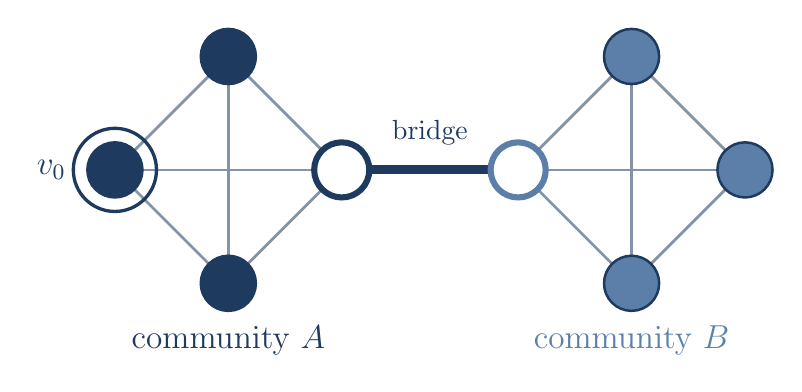
\begin{tikzpicture}[
    scale=1.6,
    node/.style={circle, minimum size=7mm, inner sep=0pt, draw=accent, line width=0.9pt},
    edge/.style={accent!55, line width=1pt}]
  \def\k{4}
  % community A (left) and B (right); node 1 of each faces the bridge
  \foreach \c/\cx/\fill/\rot in {A/-1.6/accent/0, B/1.6/accentlight/180}{
    \foreach \i in {1,...,\k}{
      \coordinate (\c\i) at ($(\cx,0)+({\rot+360*(\i-1)/\k}:0.9)$);}
    \foreach \i in {1,...,\k}{\foreach \j in {\i,...,\k}{
      \ifnum\i<\j \draw[edge] (\c\i)--(\c\j);\fi}}
    \foreach \i in {1,...,\k}{\node[node, fill=\fill] at (\c\i) {};}
  }
  % the bridge
  \draw[accent, line width=3.2pt] (A1)--(B1);
  \node[node, fill=white, line width=2.2pt] at (A1) {};
  \node[node, fill=white, draw=accentlight, line width=2.2pt] at (B1) {};
  % start node v0: interior node of A, opposite the bridge
  \draw[accent, line width=1.2pt] (A3) circle (3.3mm);
  \node[left=5mm, text=accent] at (A3) {\large $v_0$};
  % labels
  \node[text=accent, font=\large] at (-1.6,-1.35) {community $A$};
  \node[text=accentlight, font=\large] at (1.6,-1.35) {community $B$};
  \node[text=accent] at (0,0.3) {bridge};
\end{tikzpicture}
\end{document}
